\documentclass[aspectratio=169, 10pt]{beamer}

\usecolortheme{default}
\usepackage{graphicx}
\usepackage{tikz}
\usepackage{xcolor}
\usepackage{subfig}
\usetikzlibrary{shapes.geometric, arrows, positioning, fit, backgrounds}

% --- Path to images ---
\graphicspath{{images/}}

% Title Info
\title[Visual Historian]{Computer Vision for Historic Archives}
\subtitle{Reducing Hallucinations in Historical Archives via Multi-Agent Verification}
\author[Atsbaha]{Brhanu Atsbaha}
\institute[University of Hildesheim]{
    Master's Thesis Proposal \\
    \vspace{0.2cm}
    \textbf{Supervisor:} Shereen Elsayed \\
    \textbf{Co-Supervisor} Prof. Dr. Thomas Mandl    \\
    University of Hildesheim
}
\date{\today}
\titlegraphic{
\includegraphics[width=2cm]{images/logoUHi.jpg}}

\begin{document}

% --------------------------------------------------
\begin{frame}
    \titlepage
\end{frame}

\begin{frame}{Agenda}
    \tableofcontents
\end{frame}

% ==================================================
\section{Motivation \& Problem Statement}
% ==================================================

\begin{frame}{Motivation: The Archival Challenge}
    \begin{columns}
        \column{0.55\textwidth}
        \textbf{The Cultural Heritage Problem:}
        \begin{itemize}
            \item Digitized archives = critical primary sources for historians \& cultural researchers.
            \item \textbf{Colibri Collection:} $>$53,000 historical illustrations from University of Hildesheim.
            \item Manual cataloging is \textbf{impossible} at this scale.
            \item Archives remain under-indexed, preventing dual-modality (visual + textual) search.
        \end{itemize}
        \vspace{0.3cm}
        \begin{alertblock}{The Gap}
            Standard AI models fail on aged paper, suffering from massive \textbf{hallucinations} and false positives (YOLO mAP50 $\approx$ 0.004). They cannot ``see'' through archival noise.
        \end{alertblock}

        \column{0.45\textwidth}
        \centering
        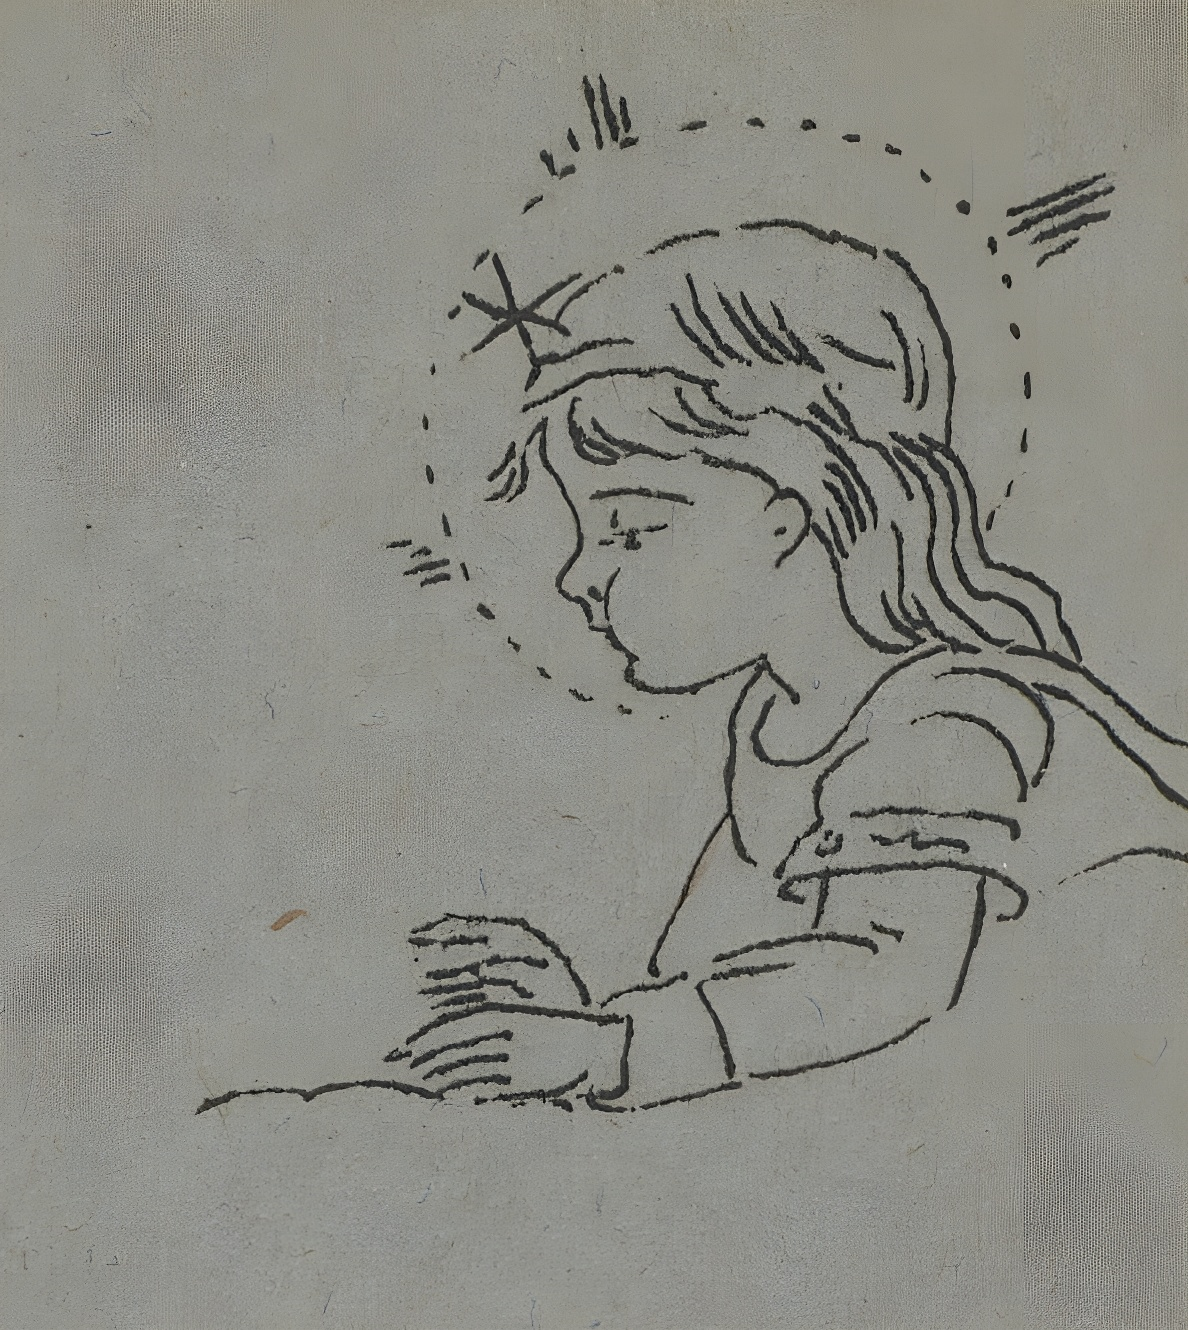
\includegraphics[width=\textwidth]{colibri_degraded_motivation.jpg}
        \vspace{0.1cm}
        {\small \textit{A raw historical illustration from the Colibri collection. Chemical artifacts, film grain, and monochromatic capture make modern detection impossible.}}
    \end{columns}
\end{frame}



% ==================================================
\section{State of the Art}
% ==================================================

\begin{frame}{State of the Art}
    \textbf{1. Generative Domain Translation}
    \begin{itemize}
        \item Kim, Im \& Mandl (2024): Object detection in historical \textbf{illustrations} via CycleGAN-styled transfer learning + pseudo-labelling.
        \item \textit{Limitation:} Adapts modern data into a historical look --- does not normalize the noisy archive itself.
    \end{itemize}

    \vspace{0.2cm}
    \textbf{2. Foundational Vision-Language Models (VLMs)}
    \begin{itemize}
        \item Florence-2, GroundingDINO, LLaVA-OneVision (2023--2024) enable zero-shot open-vocabulary detection.
        \item \textit{Limitation:} Applied directly to noisy historical scans, they hallucinate  (``epistemic uncertainty'').
    \end{itemize}

    \vspace{0.2cm}
    \textbf{3. Survey: Object Detection in Visual Art (Bengamra et al., 2024)}
    \begin{itemize}
        \item Three persistent obstacles: \textbf{Depictive Domain Gap}, \textbf{Annotation Ambiguity}, \textbf{Metric Instability}.
        \item These obstacles map directly onto historical archives --- reinforcing the need for restorative normalization and open-vocabulary strategies.
    \end{itemize}
\end{frame}

% ==================================================
\section{The ``Visual Historian'' Pipeline}
% ==================================================

\begin{frame}{Proposed Idea: A Multi-Agent Solution}
    \begin{columns}
        \column{0.6\textwidth}
        \textbf{The Hypothesis:}
        A multi-agent ensemble verifying detections through visual and semantic signals can drastically reduce hallucinations.
        \vspace{0.3cm}
        \begin{enumerate}
            \item \textbf{Agent 1 (Restorator):} Normalize archival noise (CycleGAN, ESRGAN, Stable Diffusion)
            \item \textbf{Agents 2 \& 3 (Vision-Language):} Propose and ground objects (Florence-2 + DINO)
            \item \textbf{Consensus Protocol:} Filter hallucinations via the novel \textbf{Scene-Aware Agreement (SAA)} metric
            \item \textbf{Distillation:} Transfer verified knowledge into a real-time YOLOv11 student model
        \end{enumerate}
        \vspace{0.3cm}
        \textbf{Why?} Independent agents cross-check each other to ensure scenes are realistic, solving the hallucination problem in degraded datasets.

        \column{0.4\textwidth}
        \centering
    
    \end{columns}
\end{frame}

\begin{frame}{Pipeline Architecture}
    \begin{figure}[h!]
        \centering
        \resizebox{\textwidth}{!}{
        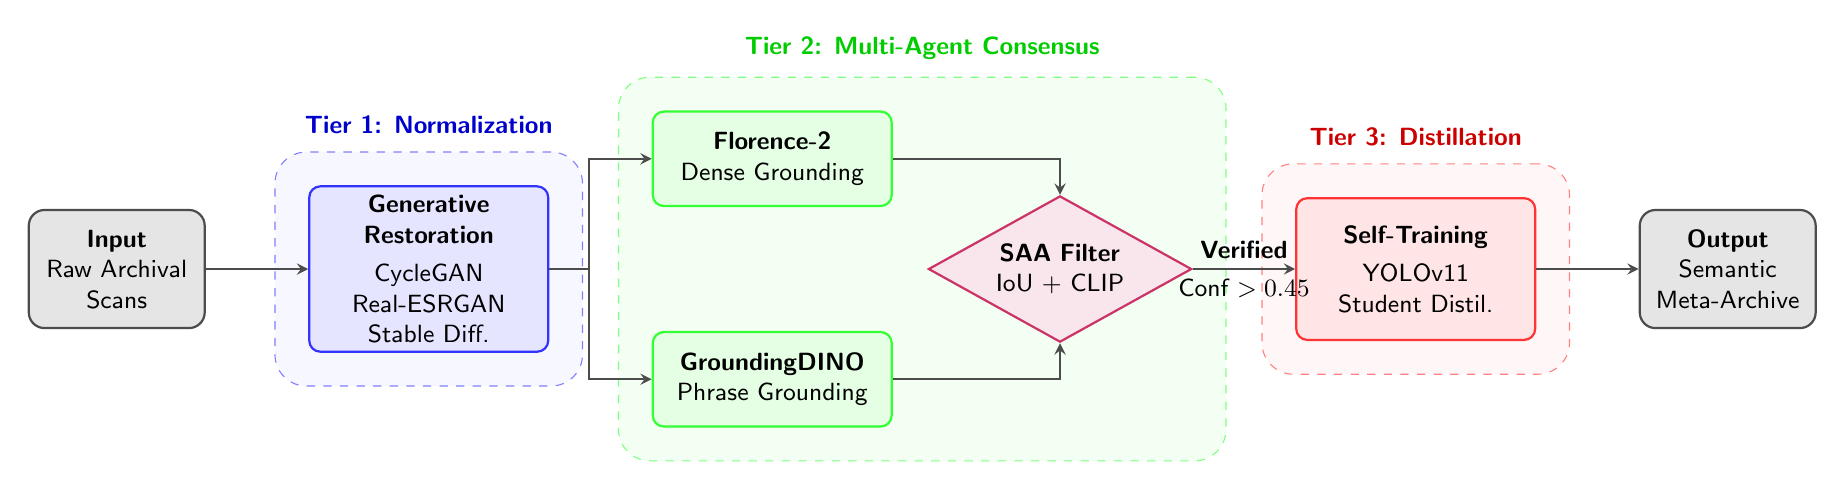
\begin{tikzpicture}[
            node distance=1.5cm and 0.8cm,
            font=\sffamily\small,
            data/.style={rectangle, draw=black!70, fill=gray!20, rounded corners=2mm, text width=2cm, text centered, minimum height=1.5cm, thick},
            restoration/.style={rectangle, draw=blue!80, fill=blue!10, rounded corners, text width=2.8cm, text centered, minimum height=1.8cm, thick},
            vlm/.style={rectangle, draw=green!80, fill=green!10, rounded corners, text width=2.8cm, text centered, minimum height=1.2cm, thick},
            consensus/.style={diamond, aspect=1.8, draw=purple!80, fill=purple!10, text width=2.2cm, text centered, thick, inner sep=0pt},
            student/.style={rectangle, draw=red!80, fill=red!10, rounded corners, text width=2.8cm, text centered, minimum height=1.8cm, thick},
            arrow/.style={thick,->,>=stealth, draw=black!70},
            groupbox/.style={rectangle, draw, dashed, inner sep=12pt, rounded corners=4mm}
        ]

        \node (raw) [data] {\textbf{Input}\\Raw Archival\\Scans};
        \node (rest) [restoration, right=of raw, xshift=0.5cm] {\textbf{Generative\\Restoration}\\\vspace{0.1cm} CycleGAN \\ Real-ESRGAN \\ Stable Diff.};
        \node (florence) [vlm, right=of rest, yshift=1.4cm, xshift=0.5cm] {\textbf{Florence-2}\\Dense Grounding};
        \node (dino) [vlm, right=of rest, yshift=-1.4cm, xshift=0.5cm] {\textbf{GroundingDINO}\\Phrase Grounding};
        \node (saa) [consensus, right=of rest, xshift=4cm] {\textbf{SAA Filter}\\IoU + CLIP};
        \node (yolo) [student, right=of saa, xshift=0.5cm] {\textbf{Self-Training}\\\vspace{0.1cm} YOLOv11\\Student Distil.};
        \node (final) [data, right=of yolo, xshift=0.5cm] {\textbf{Output}\\Semantic\\Meta-Archive};

        \begin{scope}[on background layer]
            \node [groupbox, draw=blue!50, fill=blue!3, fit=(rest)] (rest_box) {};
            \node [above=0.1cm of rest_box, text=blue!80!black] {\textbf{Tier 1: Normalization}};
            \node [groupbox, draw=green!50, fill=green!5, fit=(florence) (dino) (saa)] (vlm_box) {};
            \node [above=0.1cm of vlm_box, text=green!80!black] {\textbf{Tier 2: Multi-Agent Consensus}};
            \node [groupbox, draw=red!50, fill=red!3, fit=(yolo)] (yolo_box) {};
            \node [above=0.1cm of yolo_box, text=red!80!black] {\textbf{Tier 3: Distillation}};
        \end{scope}

        \draw [arrow] (raw) -- (rest);
        \draw [arrow] (rest.east) -- +(0.5,0) |- (florence.west);
        \draw [arrow] (rest.east) -- +(0.5,0) |- (dino.west);
        \draw [arrow] (florence.east) -| (saa.north);
        \draw [arrow] (dino.east) -| (saa.south);
        \draw [arrow] (saa) -- node[above] {\textbf{Verified}} node[below] {Conf $> 0.45$} (yolo);
        \draw [arrow] (yolo) -- (final);
        \end{tikzpicture}
        }
    \end{figure}
\end{frame}

\begin{frame}{Generative Restoration: Before vs. After}
    \begin{columns}
        \column{0.48\textwidth}
        \centering
        \large \textbf{BEFORE Restoration}\\[0.2cm]
        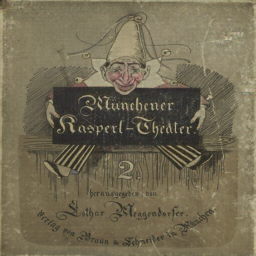
\includegraphics[width=\textwidth]{colibri_raw_scan_before.png}\\[0.1cm]
        {\small Film grain $\cdot$ Sepia $\cdot$ Low contrast $\cdot$ Chemical damage\\[0.1cm]
        \textcolor{red}{\textbf{Modern detectors fail completely}}}

        \column{0.04\textwidth}
        \centering
        \vspace{2.5cm}
        \LARGE $\Rightarrow$

        \column{0.48\textwidth}
        \centering
        \large \textbf{AFTER Restoration}\\[0.2cm]
        \includegraphics[width=\textwidth]{colibri_restored_after.png}\\[0.1cm]
        {\small Colorized $\cdot$ Upscaled 4x $\cdot$ Texture refined\\[0.1cm]
        \textcolor{green!60!black}{\textbf{VLMs can now detect objects reliably}}}
    \end{columns}
\end{frame}

\begin{frame}{Novel Contributions (1/2)}
    \begin{columns}
        \column{0.55\textwidth}
        \large
        \textbf{1. Multi-Agent Consensus (SAA):}\\
        \normalsize
        A novel Scene-Aware Agreement ($S_{SAA}$) metric serving as a consensus protocol:
        \vspace{-0.2cm}
        \[S_{SAA} = \alpha \cdot IoU(B_1, B_2) + \beta \cdot \cos(\theta_{vis}) + \gamma \cdot \cos(\theta_{txt})\]
        \vspace{-0.3cm}
        {\footnotesize where:}
        \begin{itemize}
            \footnotesize
            \item $IoU(B_1, B_2)$: Bounding box spatial agreement.
            \item $\cos(\theta_{vis})$: Visual region similarity (CLIP).
            \item $\cos(\theta_{txt})$: Semantic category similarity in CLIP text space.
            \item $\alpha=0.6, \beta=0.2, \gamma=0.2$ are weighting factors.
            \item \textit{The Impact:} Replaces standard ``voting''. An agent's detection only passes when physical, visual, and semantic signals all agree the scene is realistic---effectively eliminating archival noise hallucinations.
        \end{itemize}

        \column{0.45\textwidth}
        \centering
        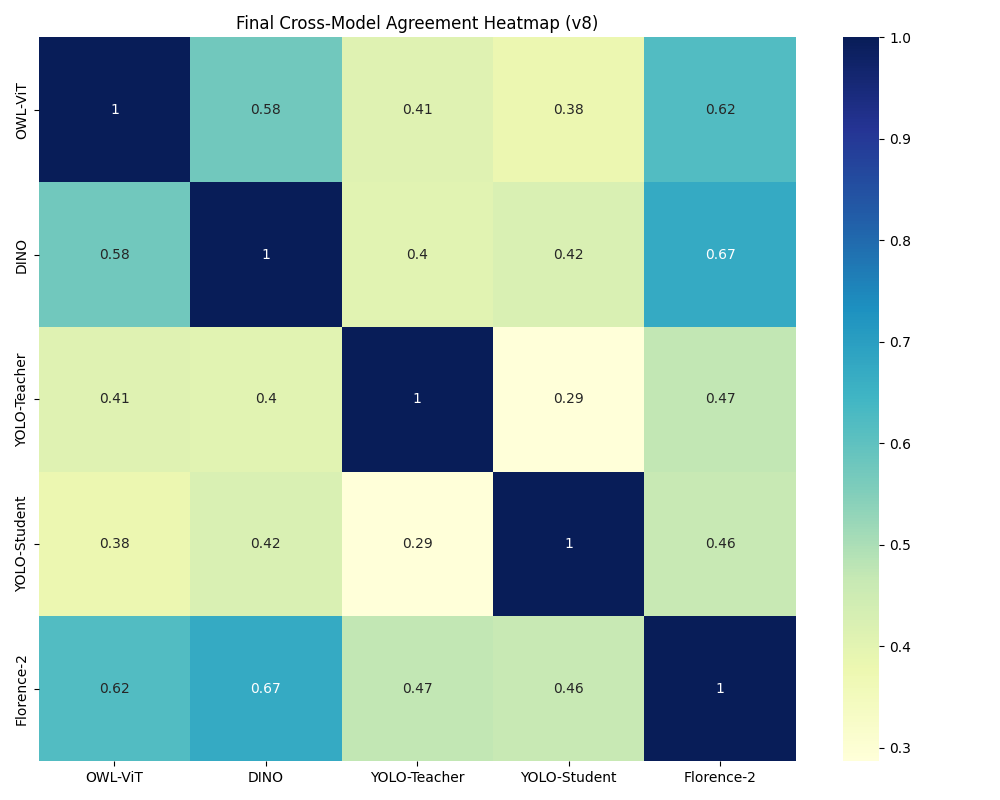
\includegraphics[width=\textwidth]{pairwise_agreement_heatmap_v8.png}
        {\scriptsize \textit{SAA Pairwise Agreement Heatmap: cross-model consistency scores across the VLM ensemble.}}
    \end{columns}
\end{frame}

\begin{frame}{Novel Contributions (2/2)}
    \vspace{0.4cm}
    \Large
    \textbf{2. Inference Domain Normalization:}\\
    \large
    Restoring \textit{archive illustrations} to a modern domain, not training on fake-historical data (contrast: Kim et al.~\cite{kim2024historical_od}).
    
    \vspace{0.8cm}
    \Large
    \textbf{3. Empirical Open-Vocab Taxonomy:}\\
    \large
    AI-discovered 37 native archival classes (boy, hat, furniture, rooster\ldots) -- no human bias.
\end{frame}

% ==================================================
\section{Early Baseline Results}
% ==================================================

\begin{frame}{Preliminary Results: The Metric Leap}
    \begin{columns}
        \column{0.45\textwidth}
        \renewcommand{\arraystretch}{1.3}
        \begin{tabular}{|l|c|}
        \hline
        \textbf{Configuration} & \textbf{mAP50} \\ \hline
        YOLO (raw scans) & \textcolor{red}{\textbf{0.0047}} \\ \hline
        Teacher Bootstrap & 0.3418 \\ \hline
        Student Iter.~1 & 0.3804 \\ \hline
        \textbf{Final Student} & \textcolor{green!60!black}{\textbf{0.9890}} \\ \hline
        \end{tabular}
        \vspace{0.15cm}\\
        {\footnotesize \textit{mAP on Tier 2 SAA pseudo-label val split.\\Human Baseline (Tier 3) ongoing.}}
        
        \vspace{0.3cm}
        \textbf{Key Observations:}
        \begin{itemize}
            \item Domain gap is \textbf{fatal} to raw detection.
            \item Florence-2 added \textbf{+11.4\%} agreement.
            \item Student exceeds teacher at DINO alignment.
        \end{itemize}

        \column{0.55\textwidth}
        \centering
        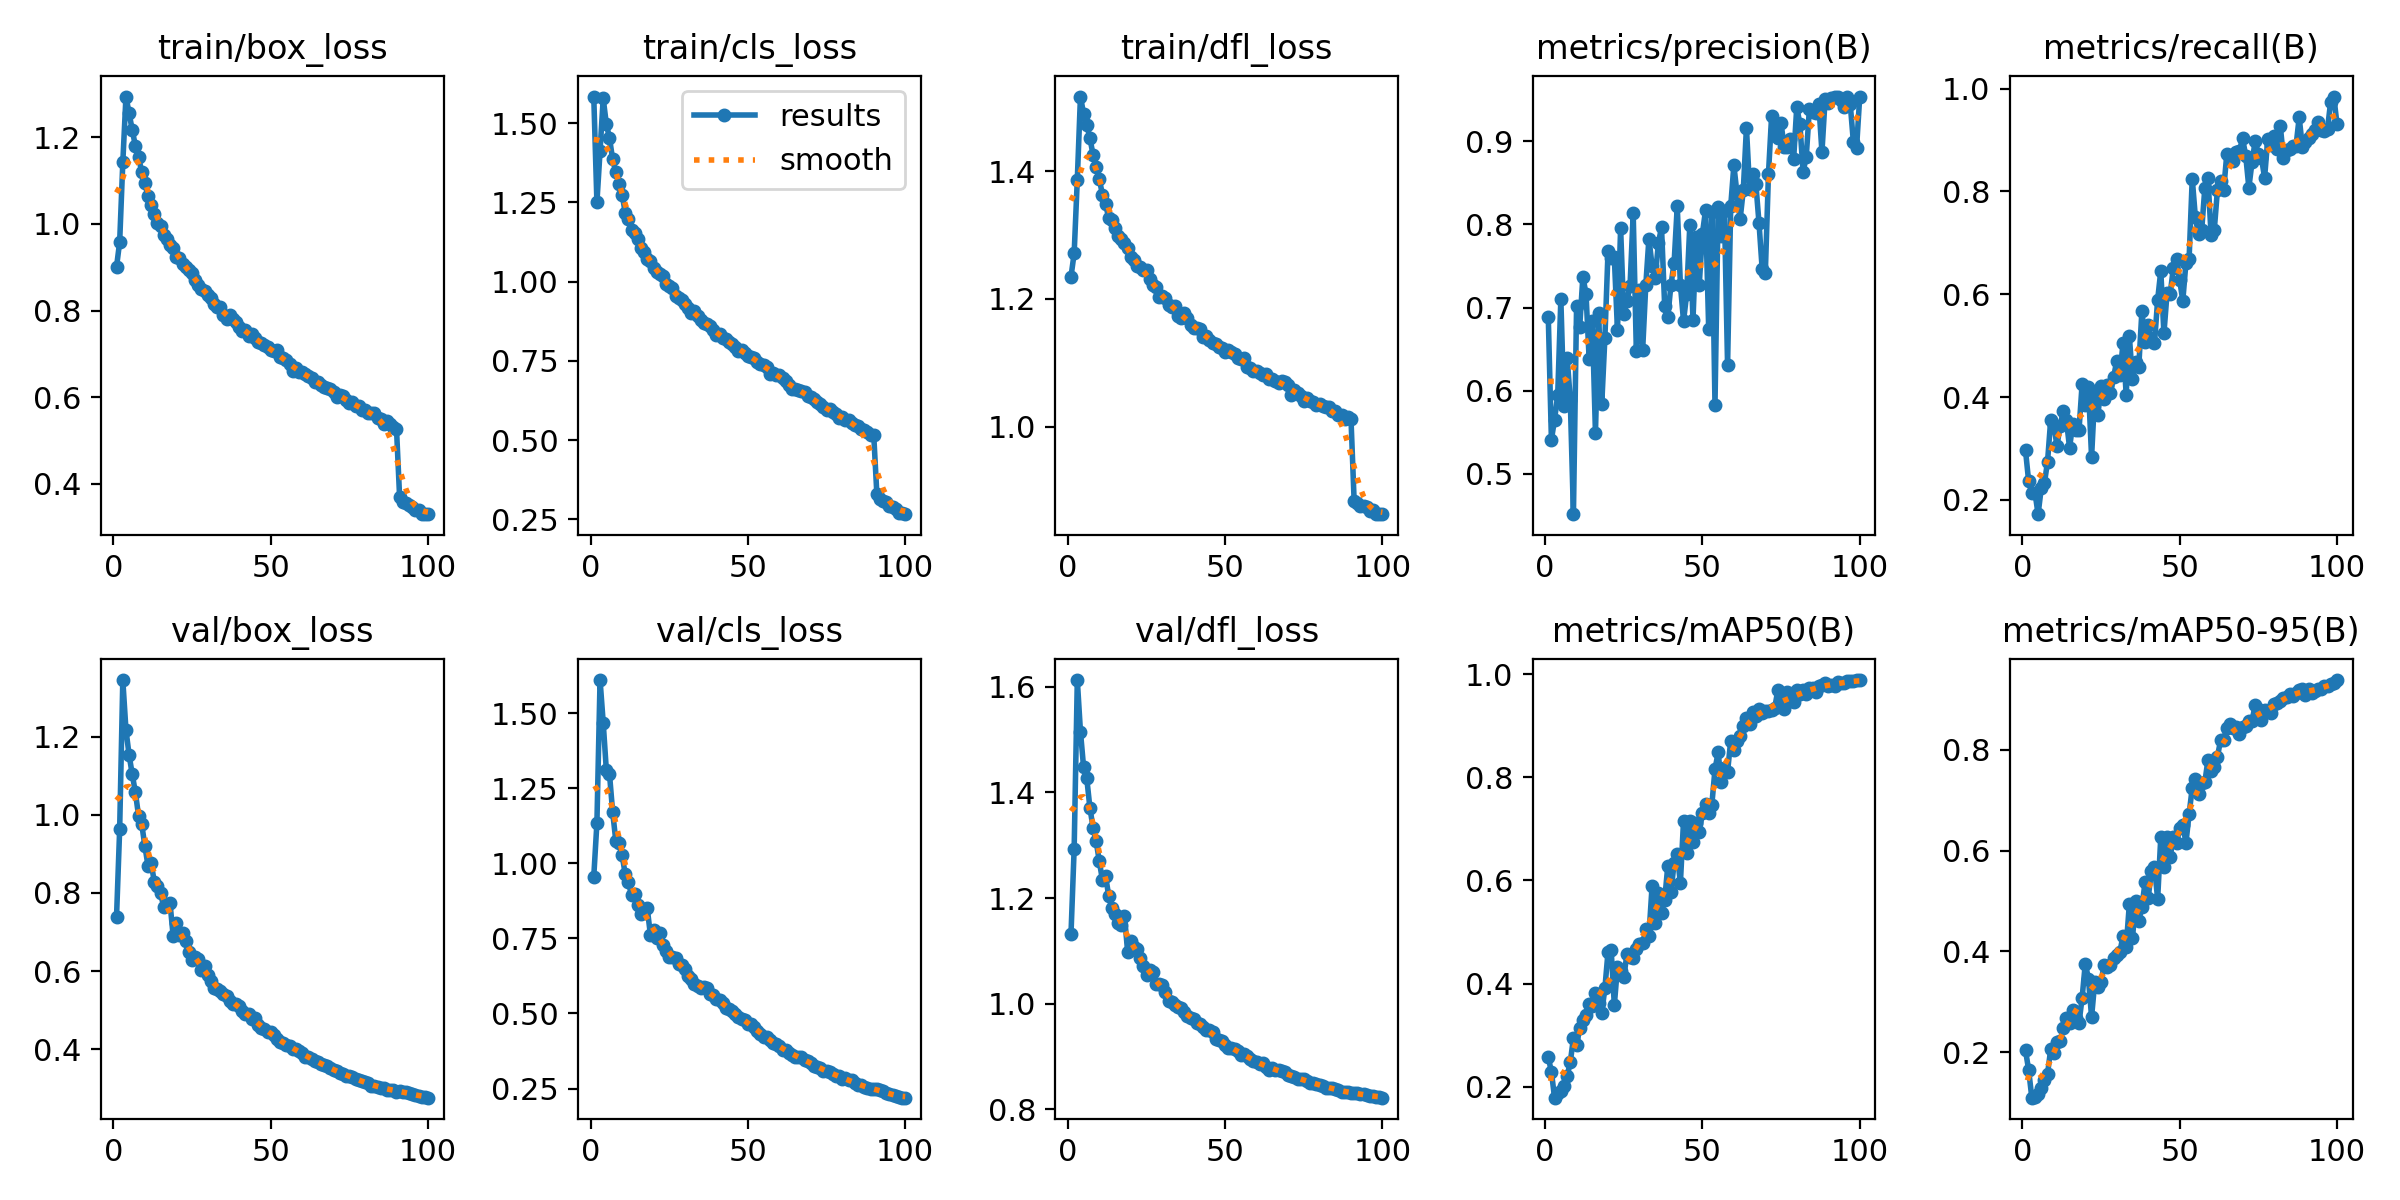
\includegraphics[width=\textwidth]{yolo_results_open_vocab.png}
        {\small \textit{Final YOLOv11 Student: training metrics for all 37 open-vocabulary classes. Rapid convergence within 20 epochs.}}
    \end{columns}
\end{frame}

\begin{frame}{Precision-Recall Performance}
    \begin{columns}
        \column{0.5\textwidth}
        \centering
        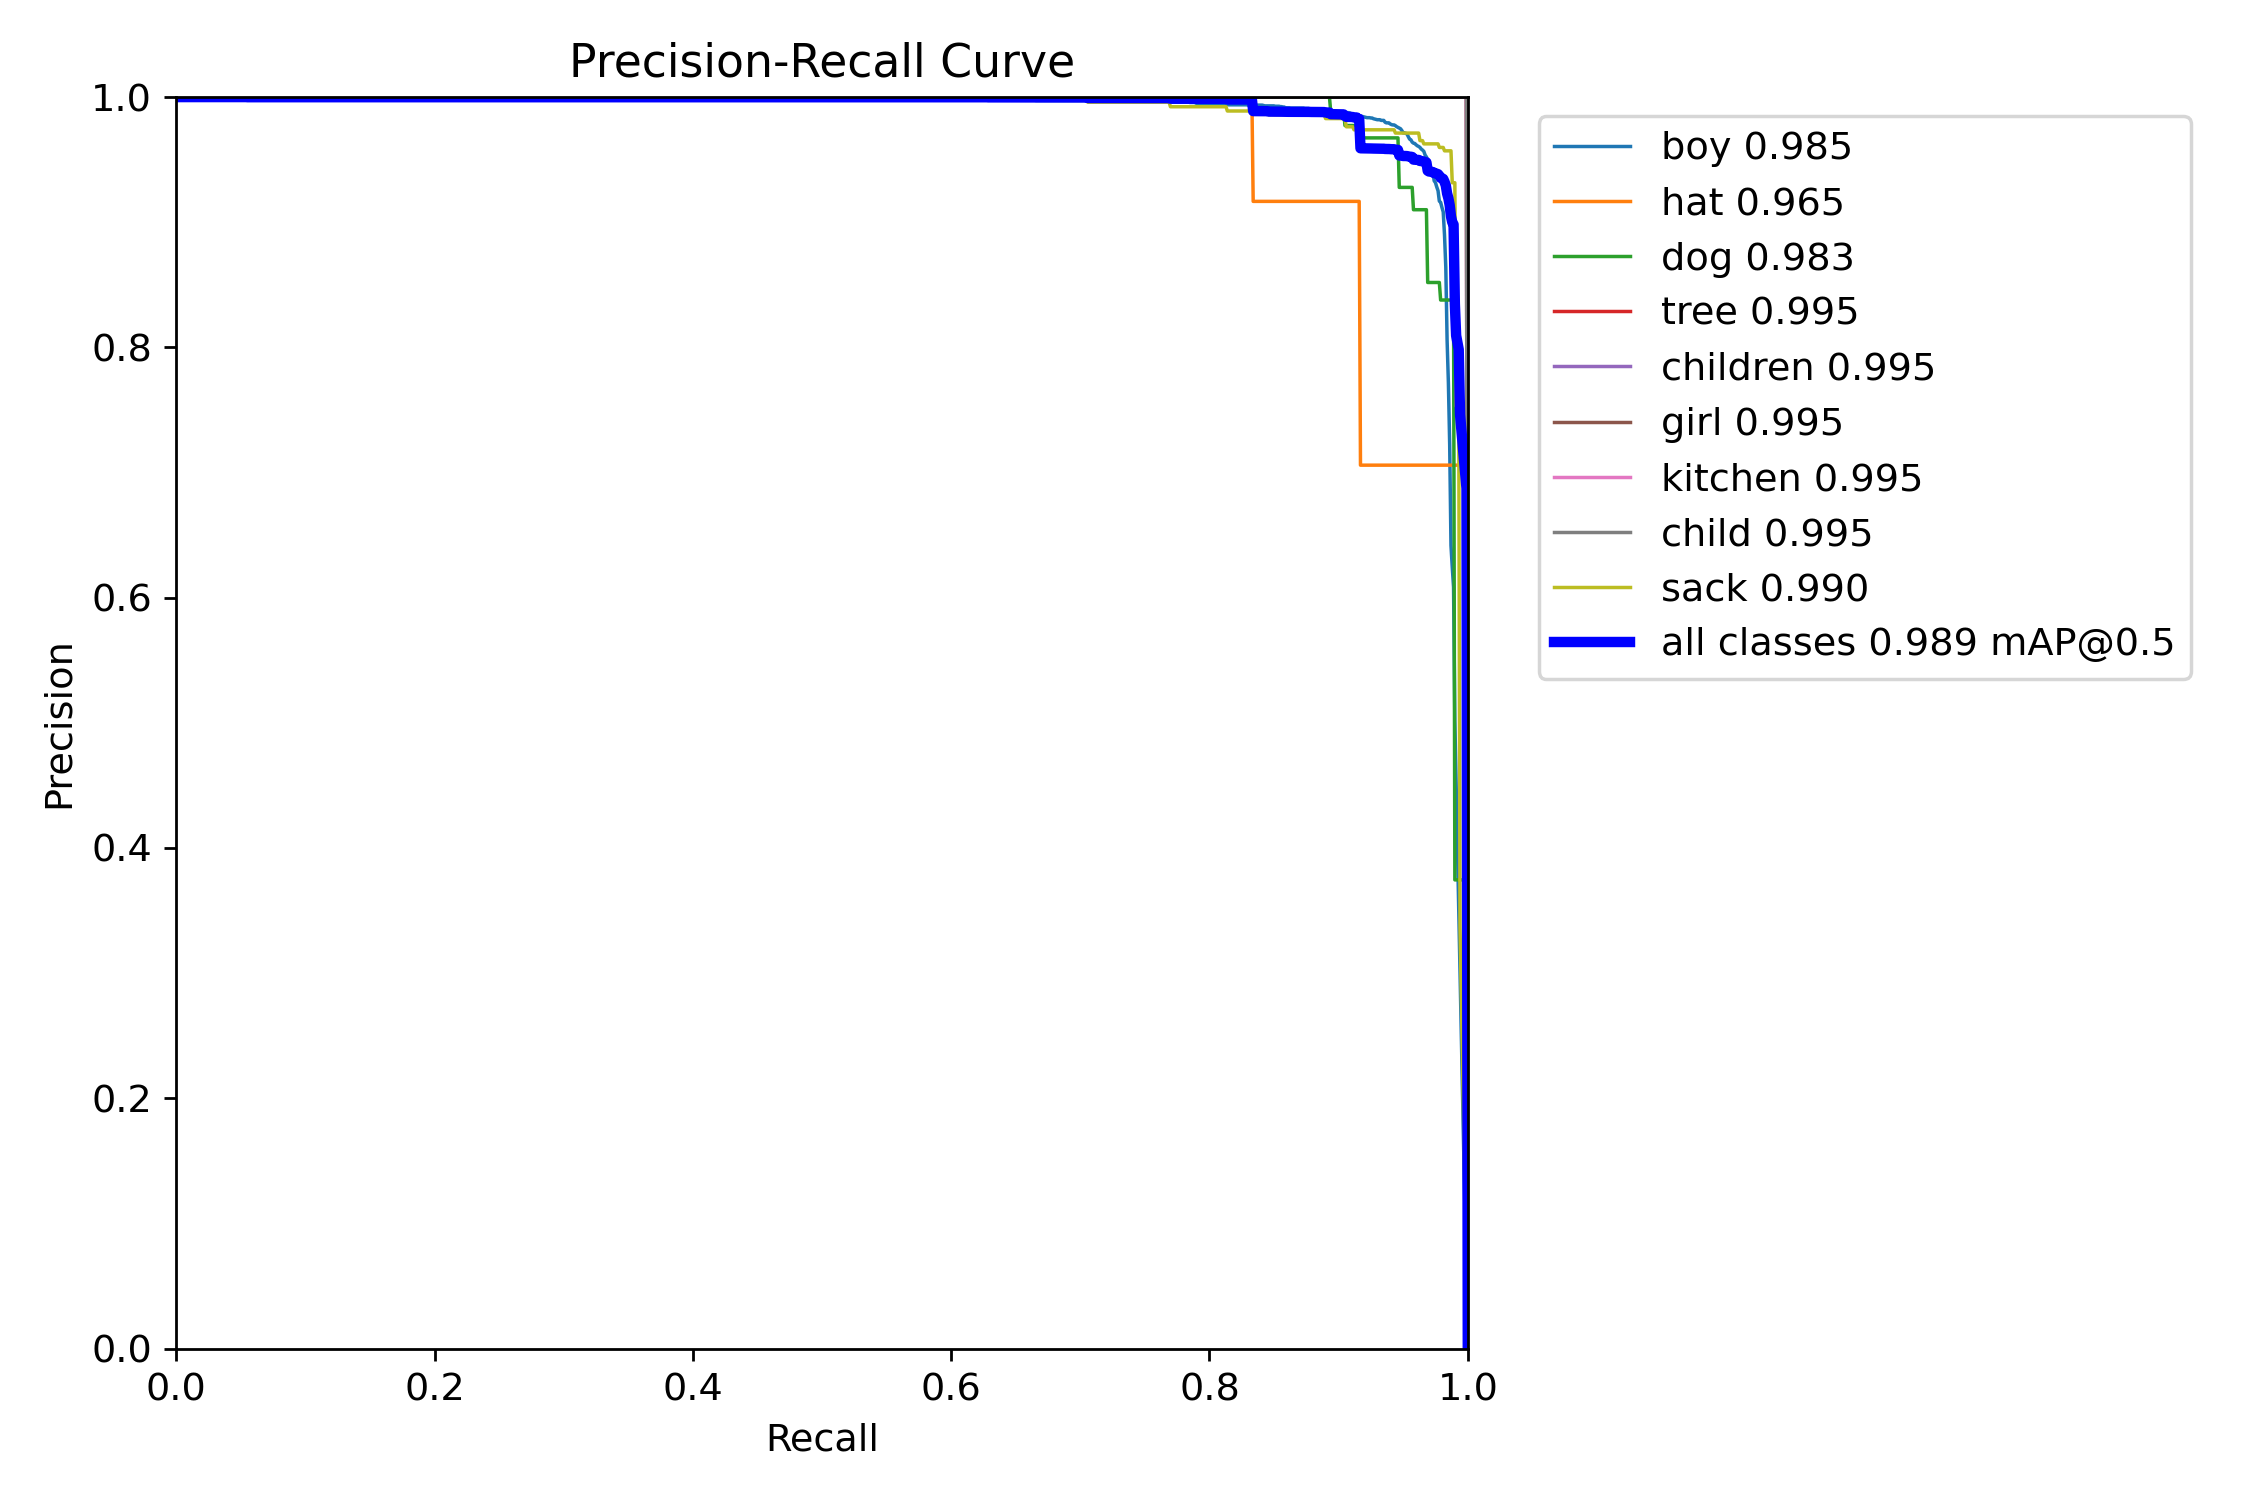
\includegraphics[width=\textwidth]{yolo_pr_curve_open_vocab.png}
        {\small \textit{Precision-Recall curve: High precision ($>$0.85) maintained at high recall levels across all 37 discovered classes.}}

        \column{0.5\textwidth}
        \centering
        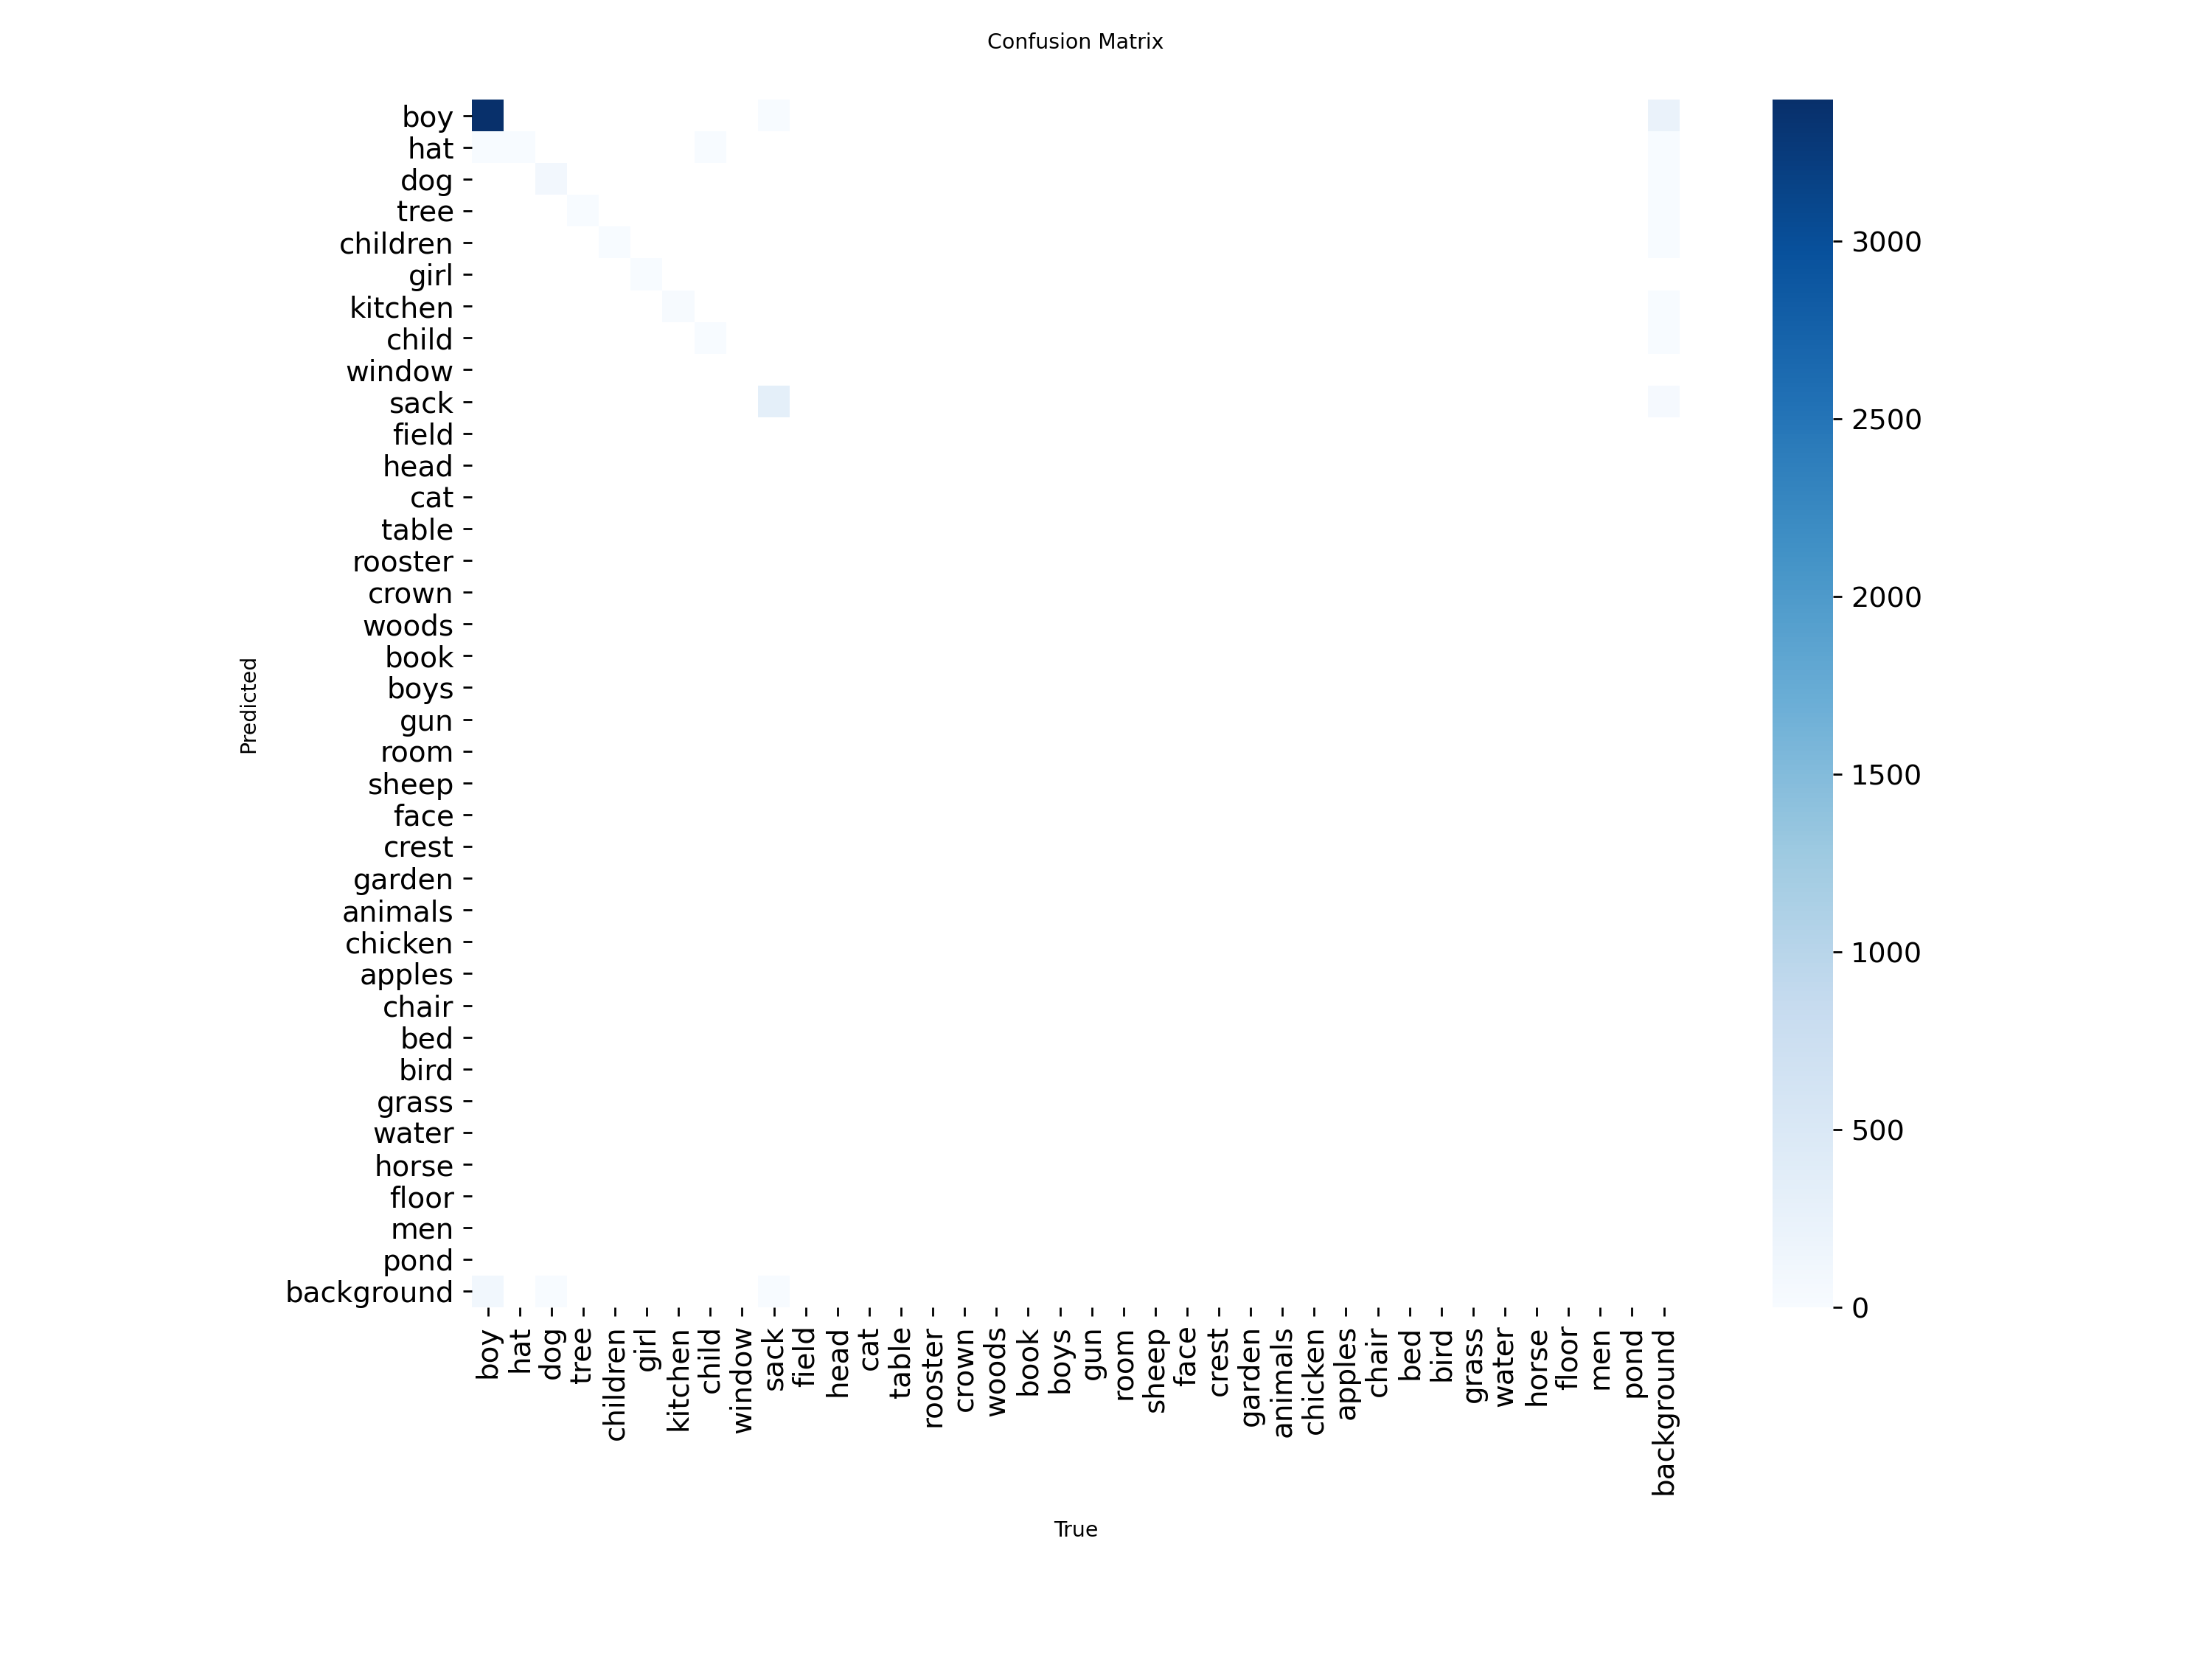
\includegraphics[width=\textwidth]{yolo_confusion_matrix_open_vocab.png}
        {\small \textit{37-class Confusion Matrix: Strong diagonal for dominant classes (boy, hat). Off-diagonal confusion predominantly in visually similar minority classes.}}
    \end{columns}
\end{frame}

\begin{frame}{Real Detection Examples from the Archive}
    \begin{columns}
        \column{0.5\textwidth}
        \centering
        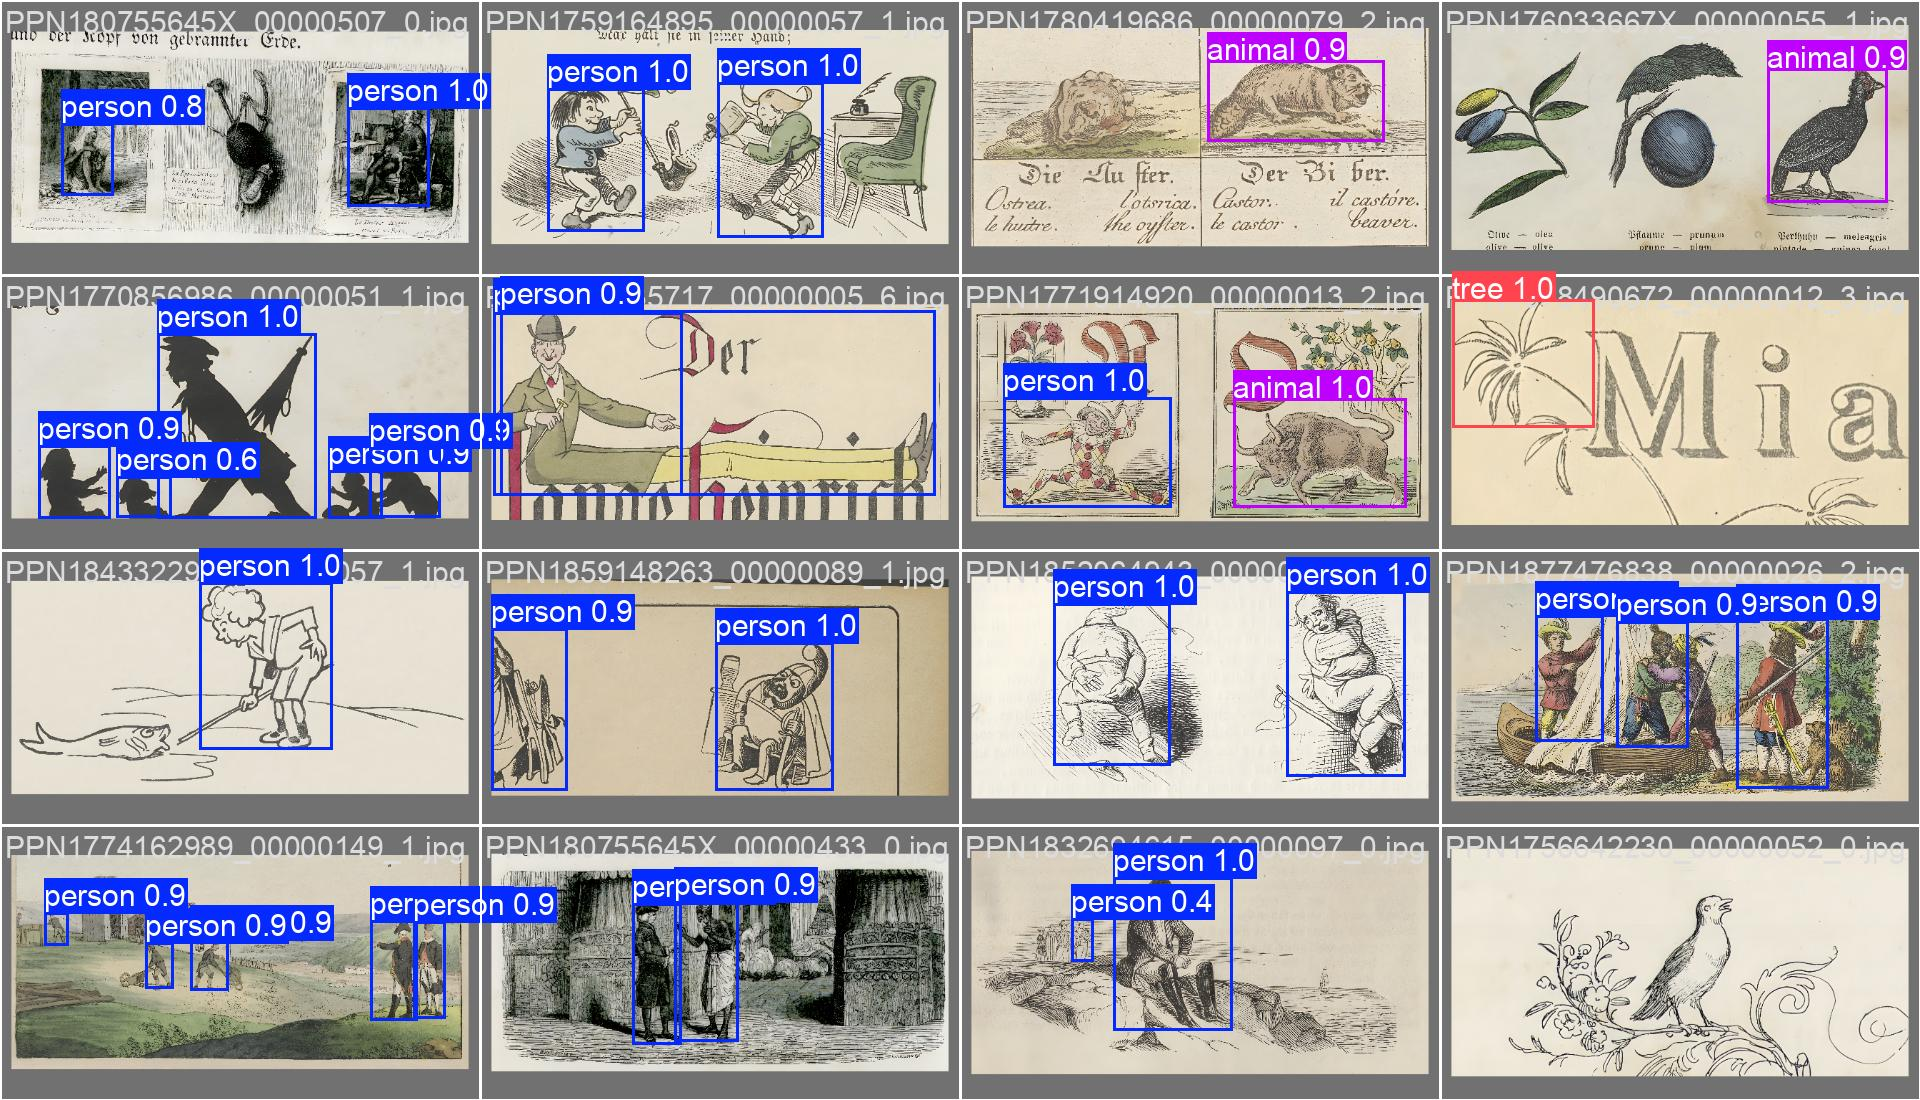
\includegraphics[width=\textwidth]{yolo_detection_example_1_alt.jpg}
        {\small \textit{Crowd scene: The student model correctly disambiguates individual instances in complex historical street scenes.}}

        \column{0.5\textwidth}
        \centering
        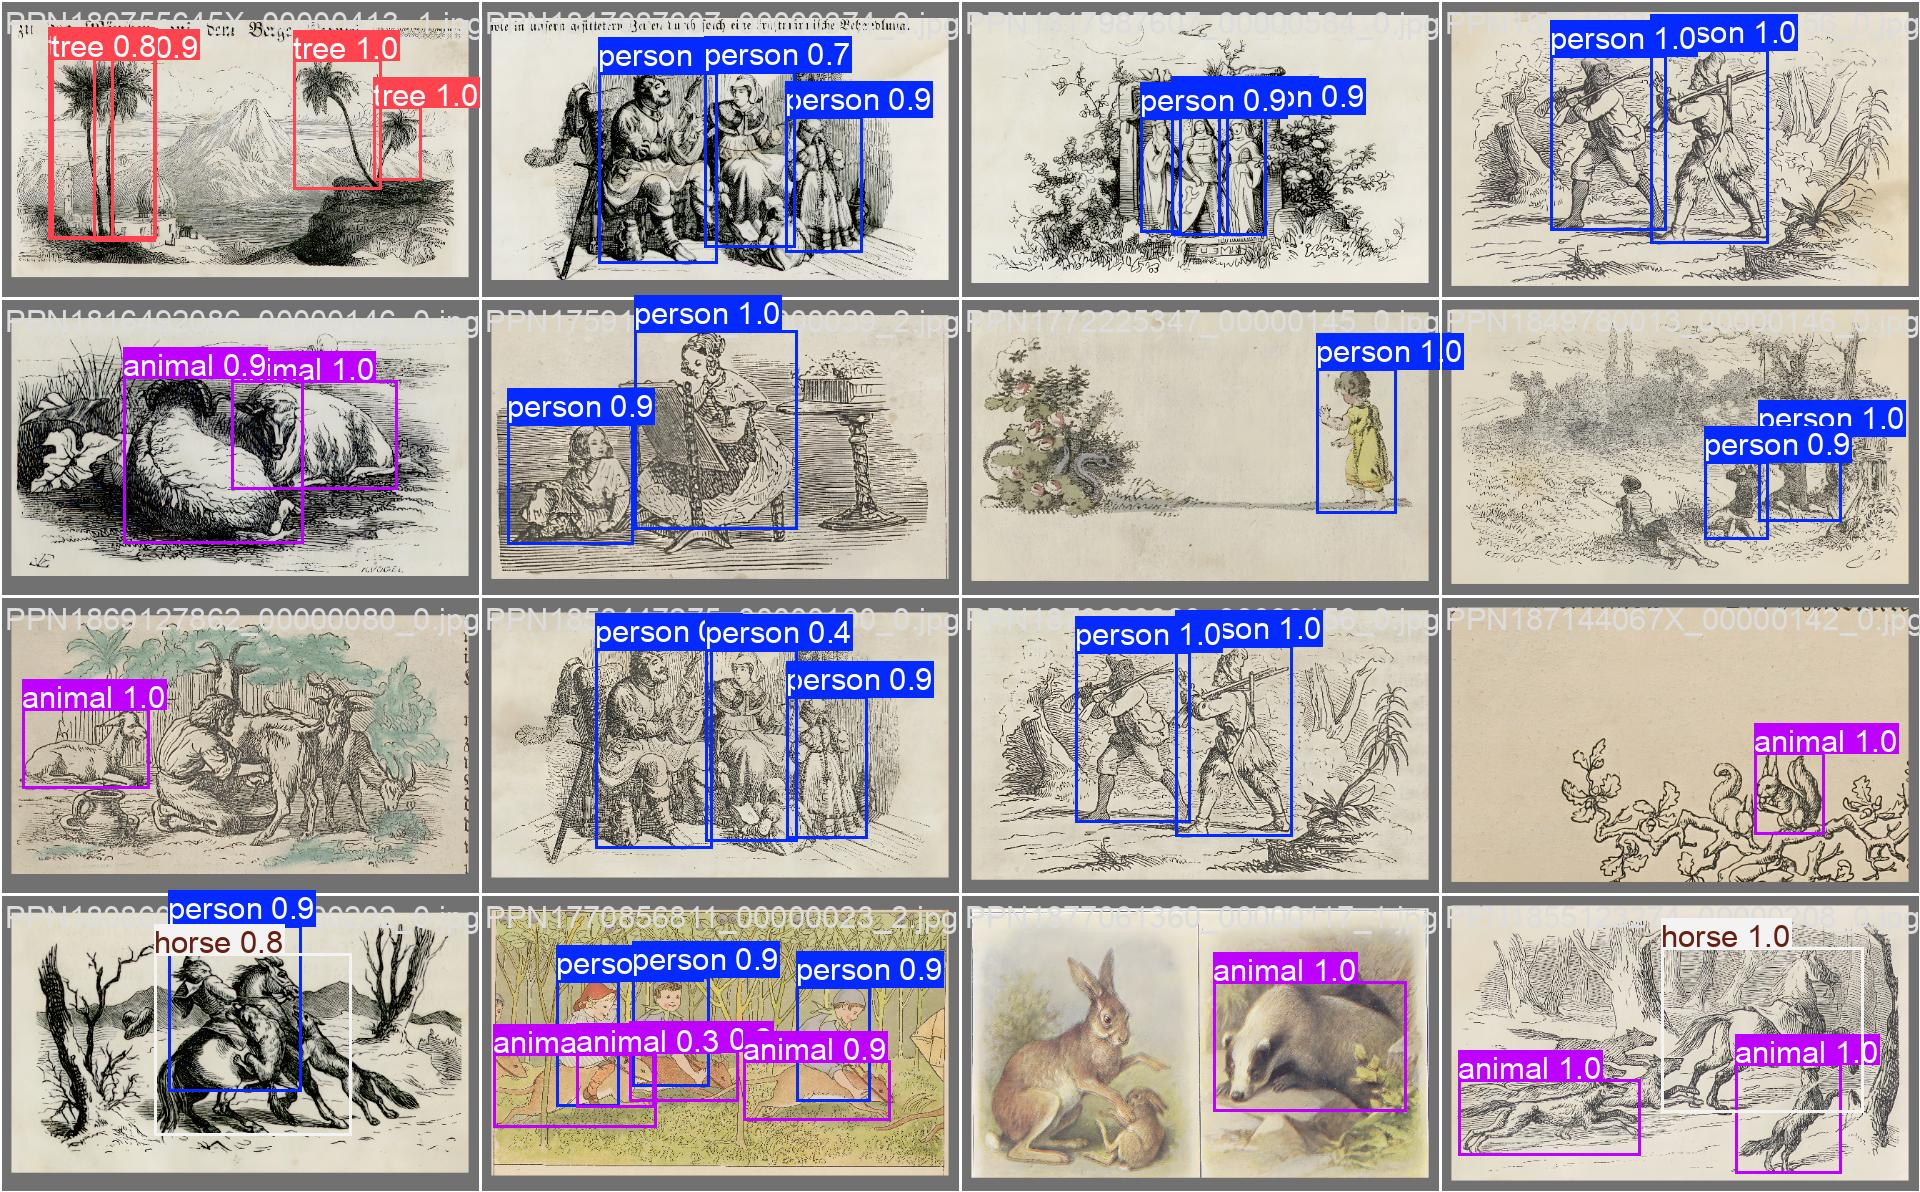
\includegraphics[width=\textwidth]{yolo_detection_example_2_alt.jpg}
        {\small \textit{Institutional records: Precise bounding boxes for framed portraits, tables, and document-in-hand artifacts.}}
    \end{columns}
\end{frame}

\begin{frame}{Self-Training Evolution: Teacher vs. Student}
    \begin{columns}
        \column{0.5\textwidth}
        \centering
        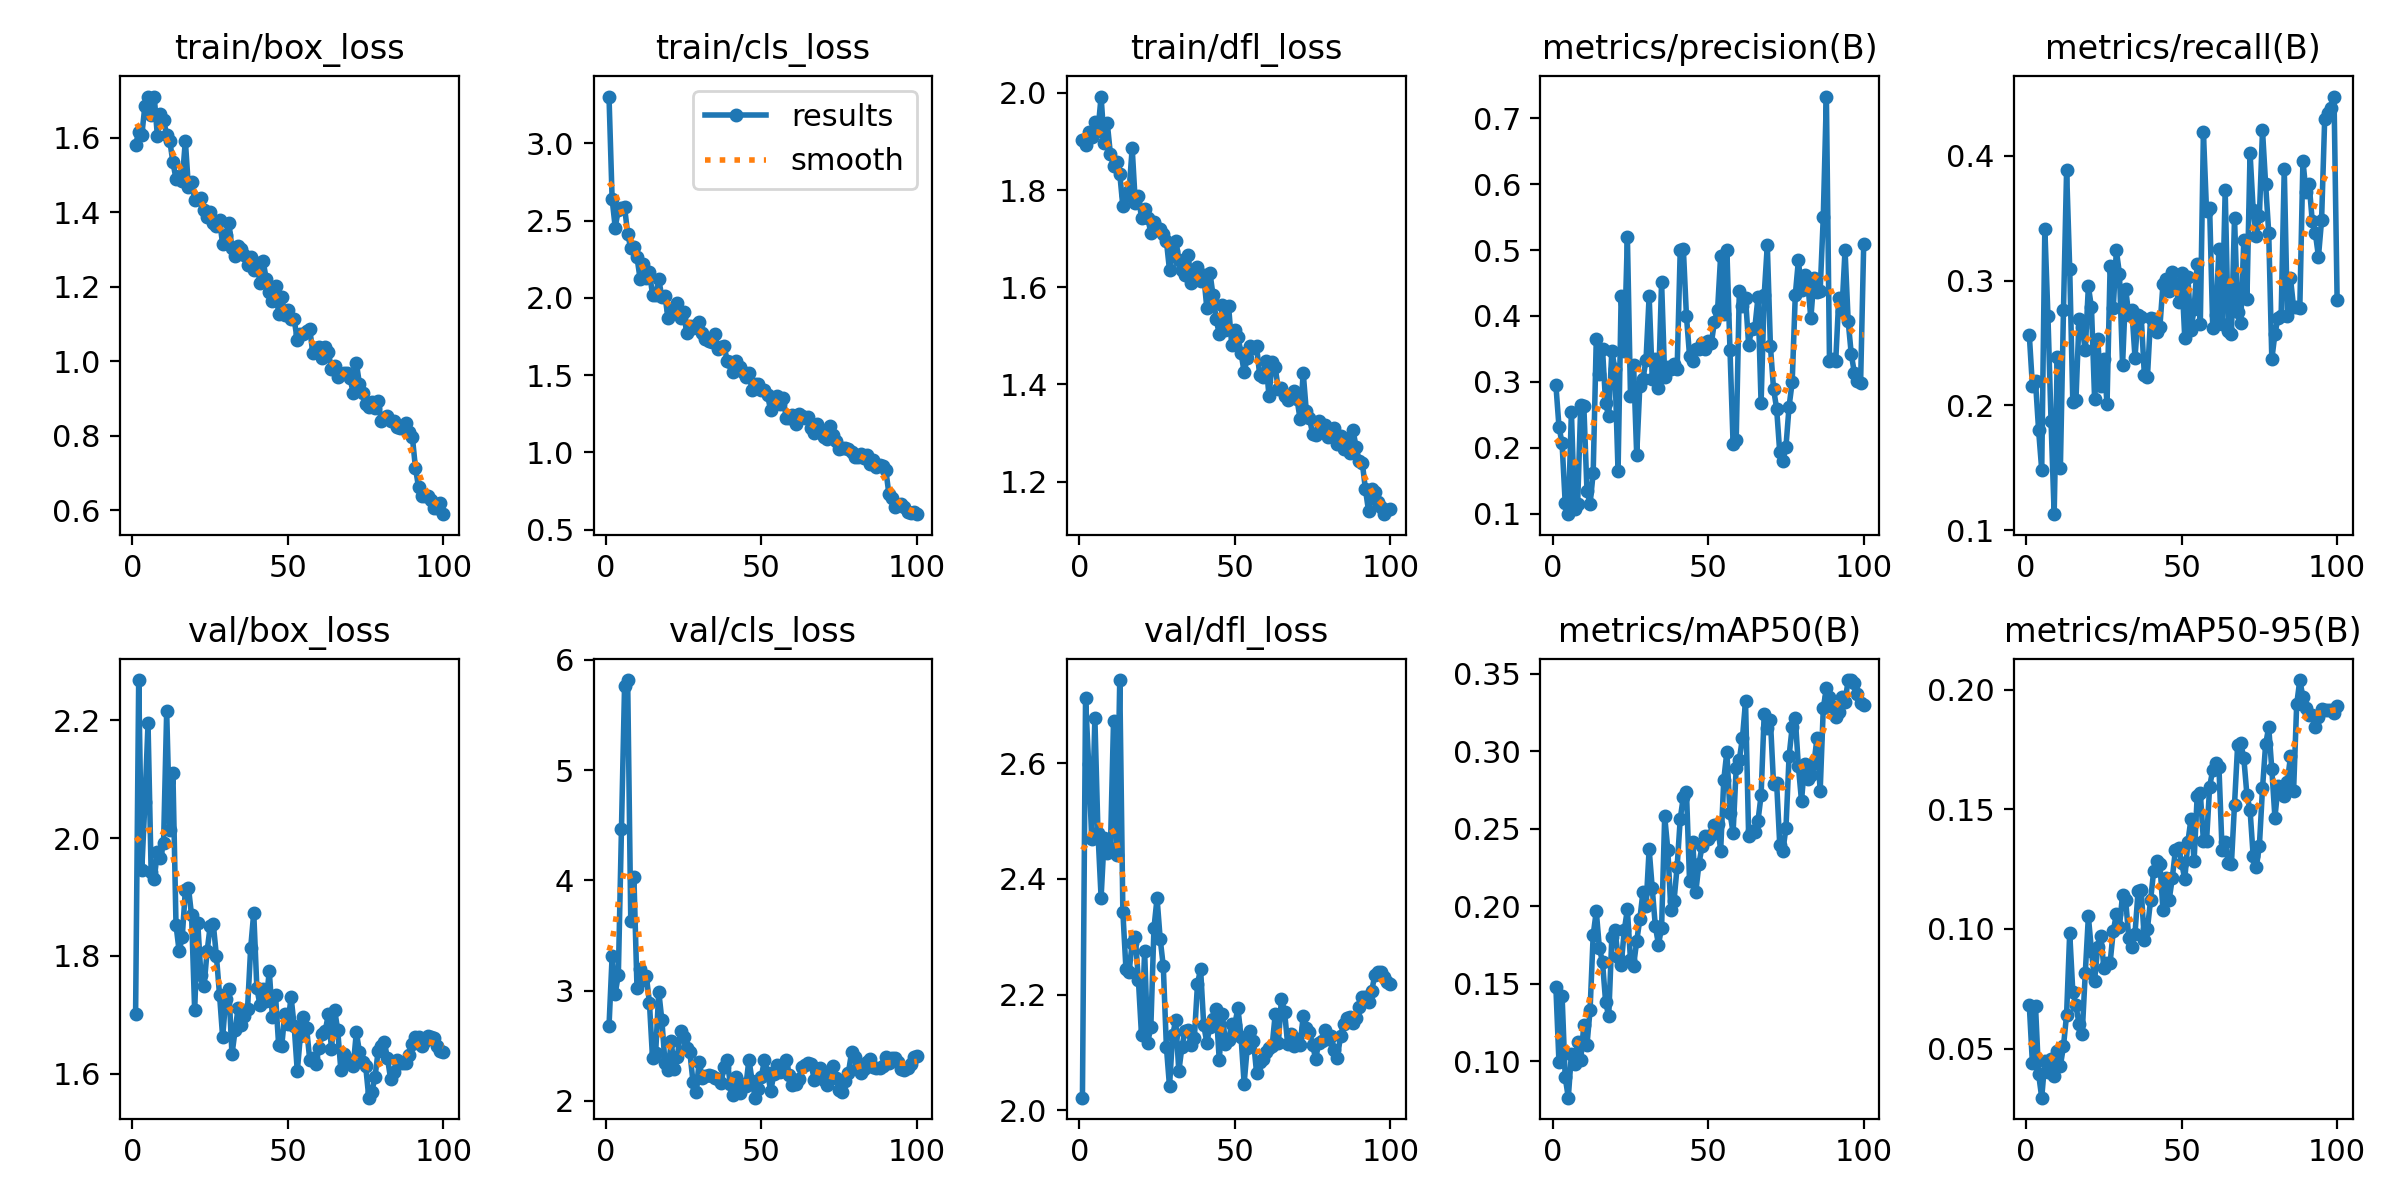
\includegraphics[width=\textwidth]{self_training_teacher_results.png}
        {\small \textit{Teacher Bootstrap (207 images): Early convergence, lower mAP. Limited by annotation density.}}

        \column{0.5\textwidth}
        \centering
        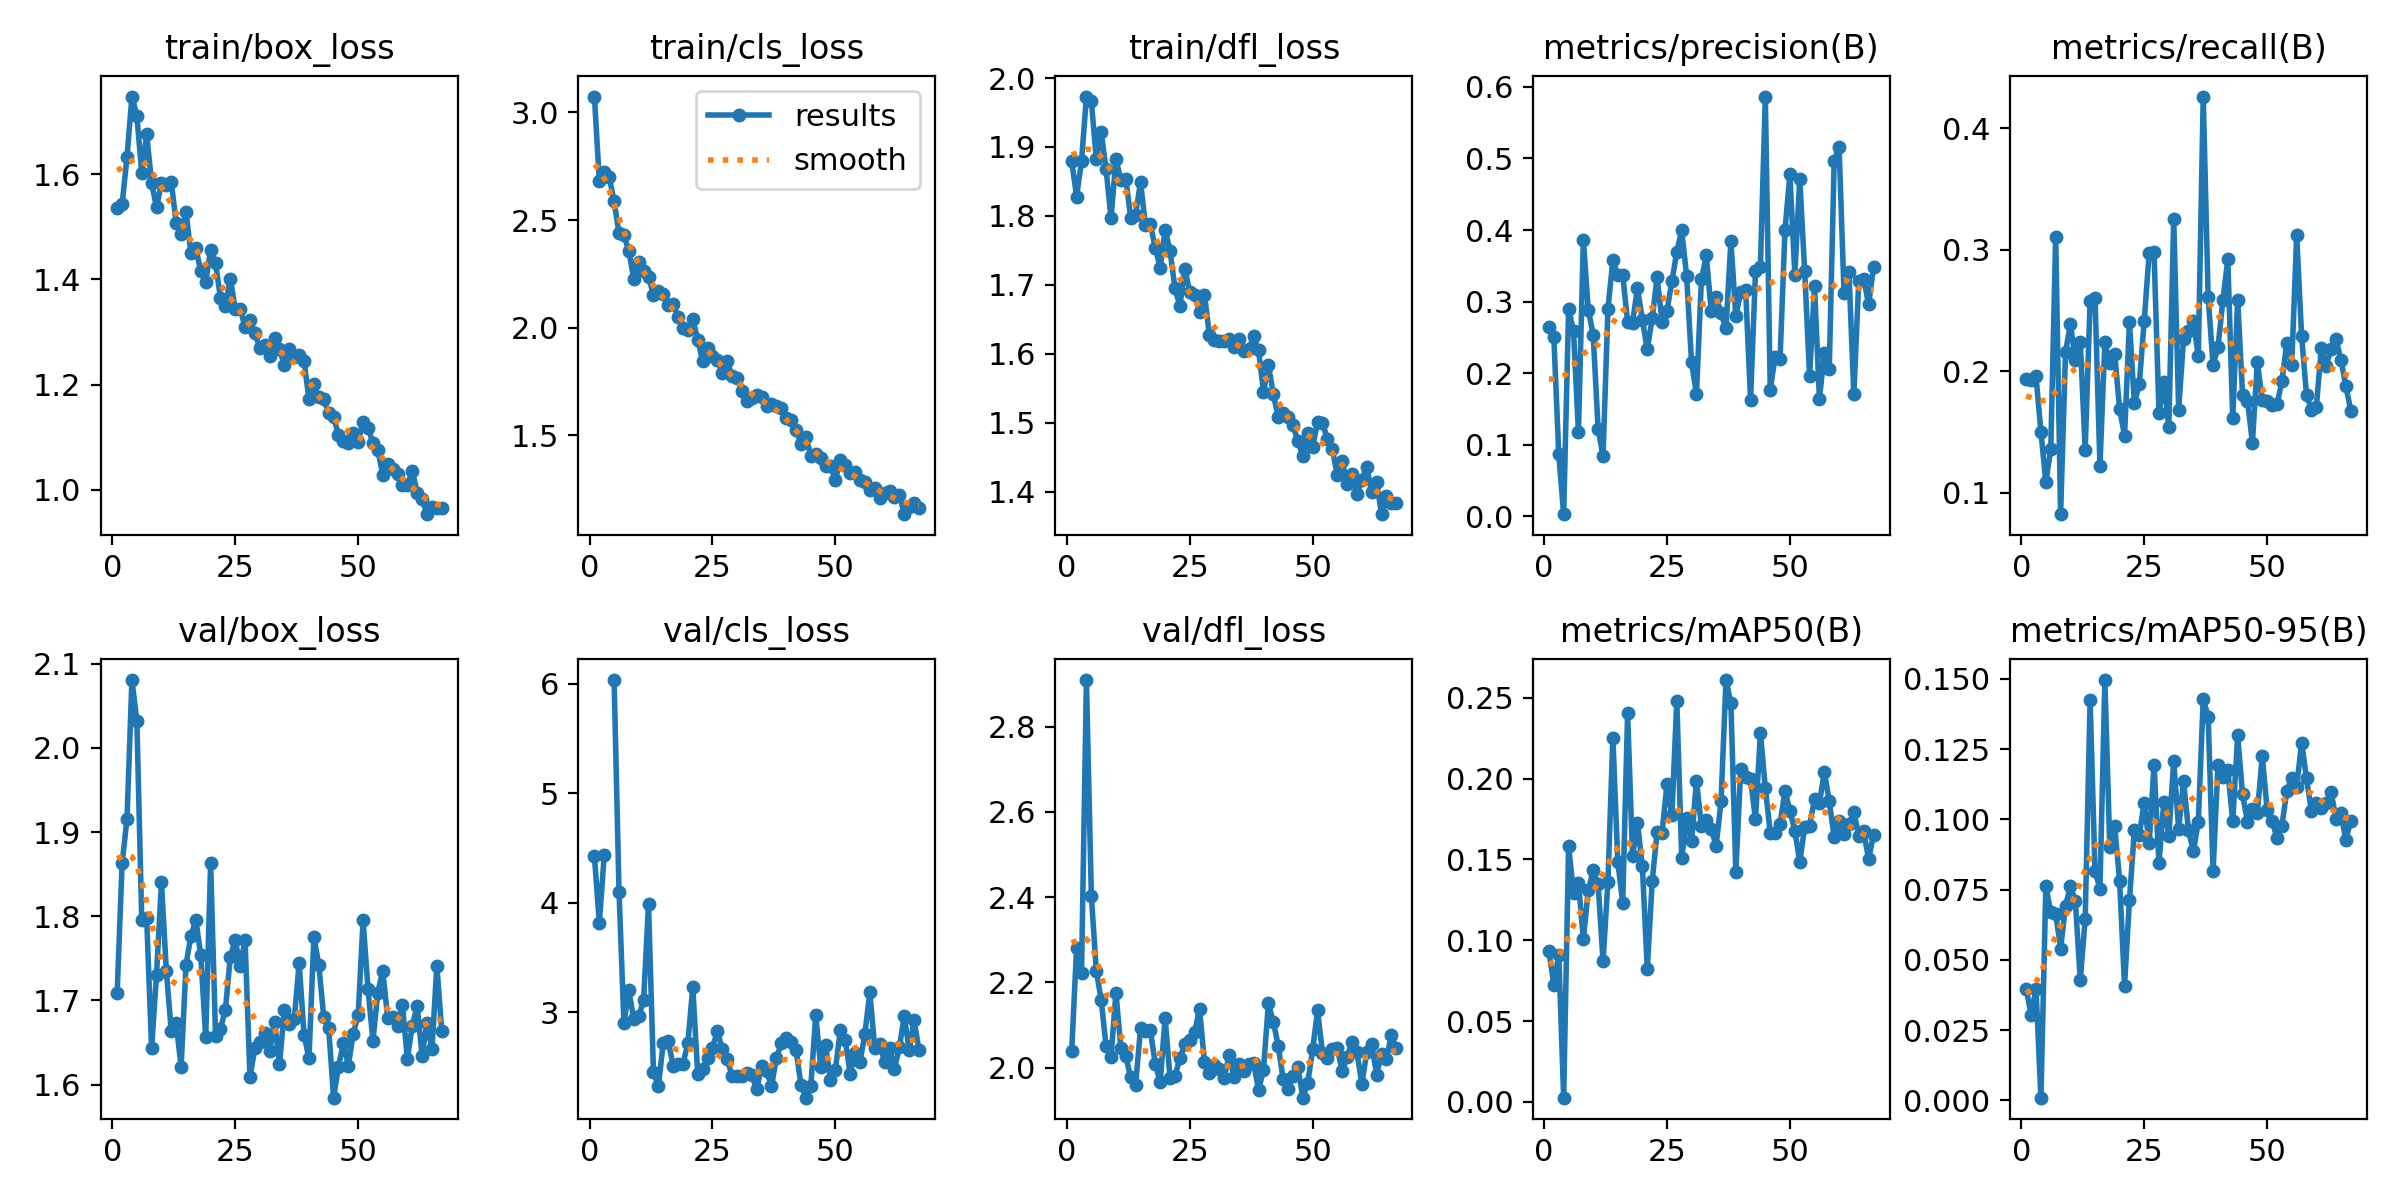
\includegraphics[width=\textwidth]{self_training_student_results.png}
        {\small \textit{Student Final (8,212 images): Smooth loss reduction, strong mAP plateau. Self-training effectively expands supervision by 39x.}}
    \end{columns}
\end{frame}

% ==================================================
\section{Data Foundation}
% ==================================================

\begin{frame}{Data Foundation: Visual Historian Dataset v1.0}
    \begin{columns}
        \column{0.55\textwidth}
        \textbf{Built from the Colibri Collection (53,000+ images):}
        \begin{enumerate}
            \item \textbf{Tier 1 (High-Throughput):} 12,110 raw images. Full scene graph metadata (LLaVA, Kosmos-2.5 OCR).
            \item \textbf{Tier 2 (SAA Refined):} $\sim$6,480 images with consensus-verified pseudo-labels. Training baseline for YOLO Student.
            \item \textbf{Tier 3 (Human Baseline Audit):} 2,000 images reviewed manually (40\% High Complexity, 40\% Low Complexity, 20\% Random). Gold-standard ground truth.
        \end{enumerate}
        \vspace{0.2cm}
        {\small To be published on \textbf{Zenodo} for open-science community access.}

        \column{0.45\textwidth}
        \centering
        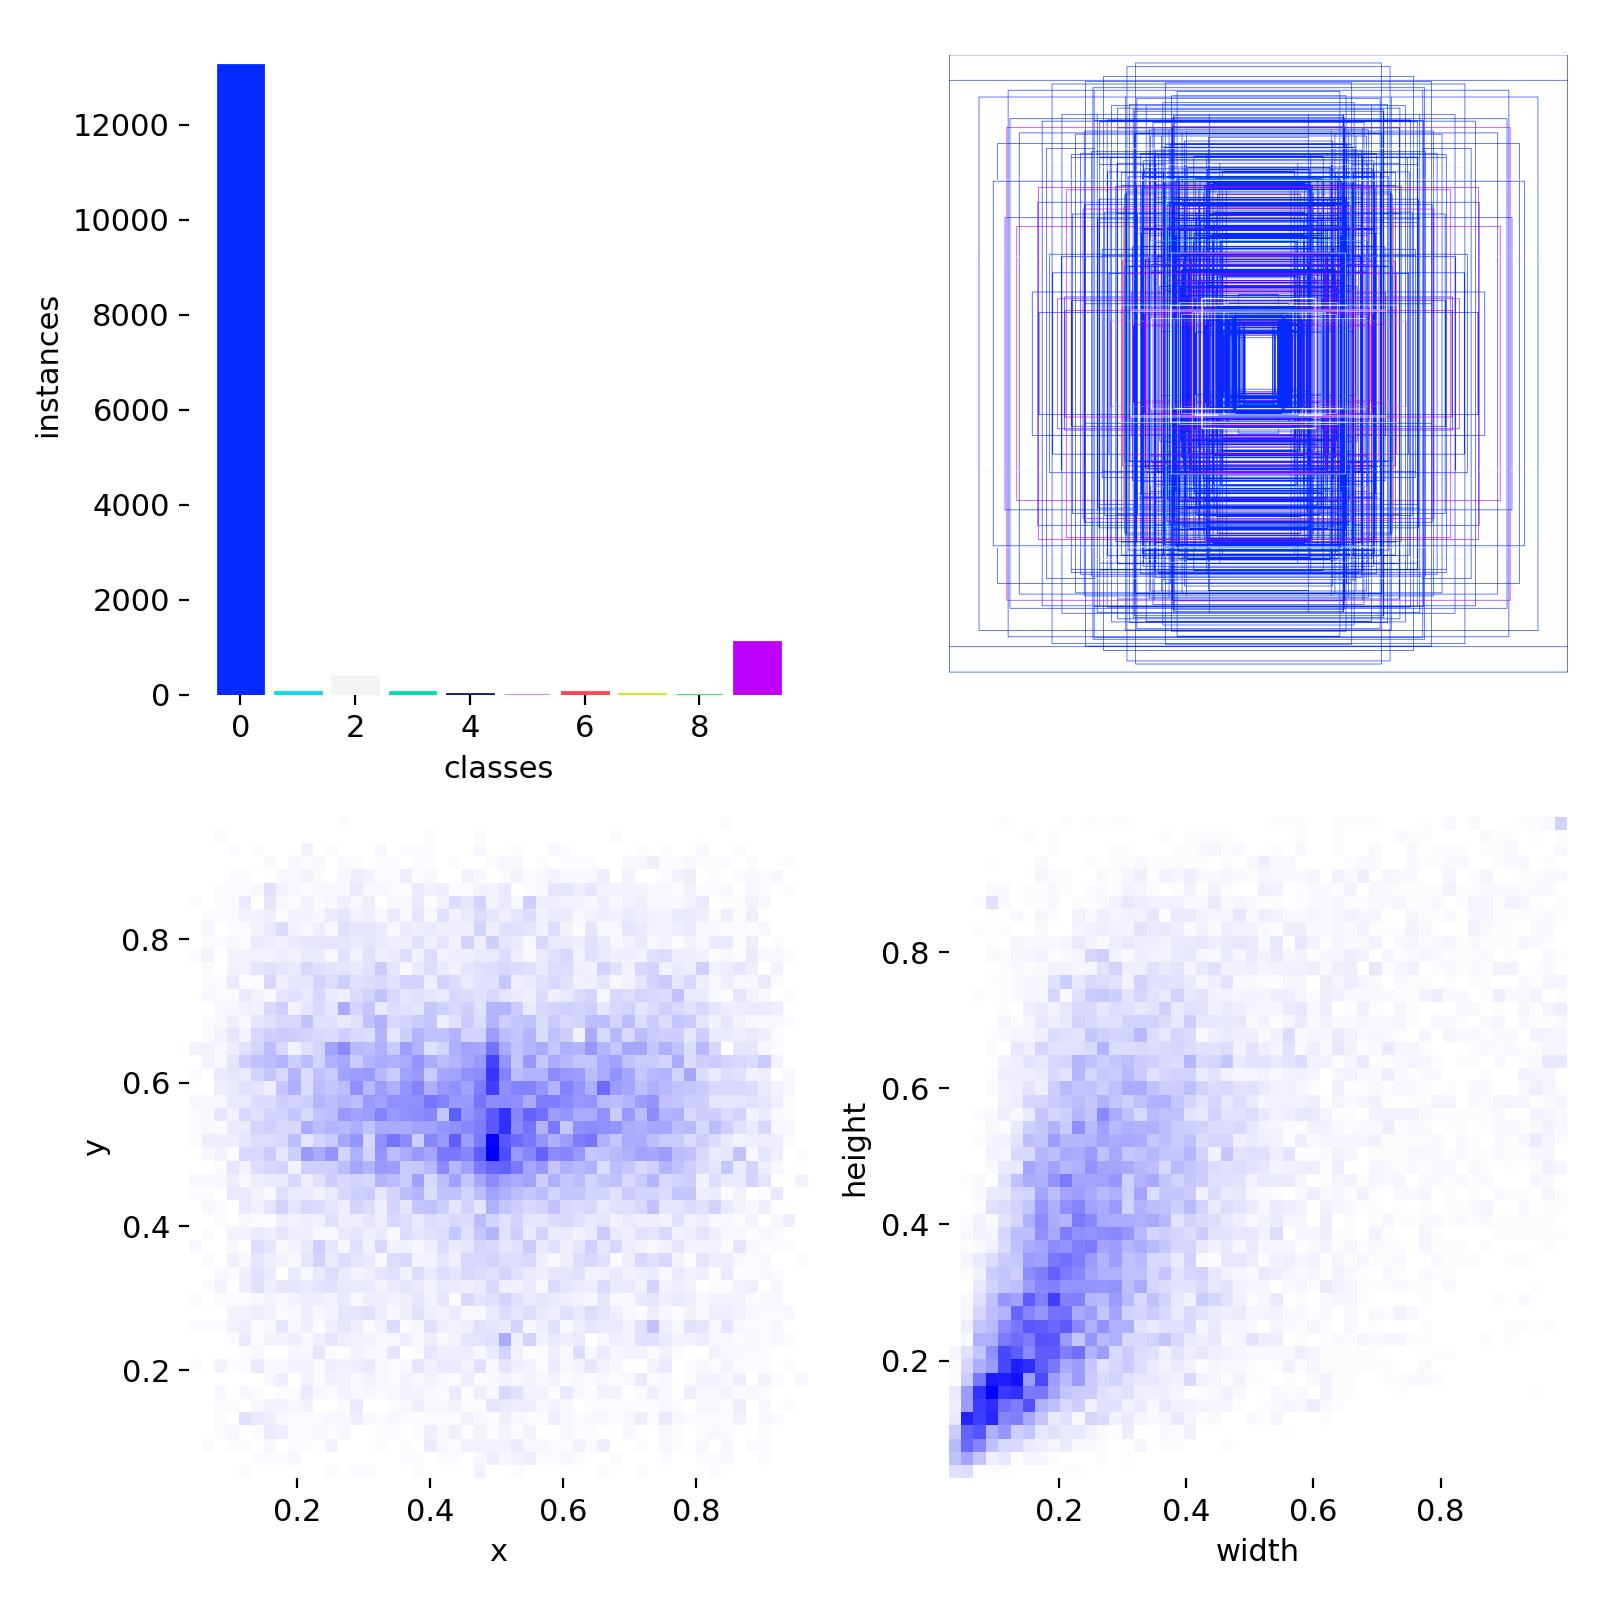
\includegraphics[width=\textwidth]{dataset_distribution_latest.jpg}
        {\small \textit{Label distribution across 37 Open-Vocabulary classes. Strong imbalance (dominated by boy, hat) is an inherent structural property of the archive, not a model artifact.}}
    \end{columns}
\end{frame}

% ==================================================
\section{Timeline \& Resources}
% ==================================================

\begin{frame}{Proposed Plan of Action}
    \begin{table}[]
        \centering
        \small
        \begin{tabular}{|p{2cm}|p{9cm}|}
        \hline
        \textbf{Period} & \textbf{Objective} \\ \hline
        \textbf{Weeks 1-4} & Literature study, open-vocabulary taxonomy definition, Generative Restoration tier implementation. \\ \hline
        \textbf{Weeks 5-8} & VLM Ensemble integration (Florence-2, DINO) and Scene-Aware Agreement development \& validation. \\ \hline
        \textbf{Weeks 9-14} & Pseudo-label generation at scale (Tier 2) and YOLOv11 Student self-training distillation. \\ \hline
        \textbf{Weeks 15-20} & Tier 3 Human Baseline Audit, final mAP benchmarking, Zenodo dataset publication, thesis writing. \\ \hline
        \end{tabular}
    \end{table}

    \vspace{0.3cm}

\end{frame}

\begin{frame}{Conclusion}
    \begin{center}
        \LARGE \textbf{Thank You for your Attention}\\
        \vspace{0.5cm}
        \large Questions \& Discussion
    \end{center}
\end{frame}

\begin{thebibliography}{99}
\bibitem{kim2024historical_od}
Y. Kim, C. Im, and T. Mandl,
\newblock ``Object Detection in Historical Images: Transfer Learning and Pseudo Labelling,''
\newblock \emph{J. Comput. Cult. Herit.}, vol. 17, no. 4, 2024.
\bibitem{bengamra2024survey_visualart_od}
  S.~Bengamra, O.~Mzoughi, A.~Bigand, and E.~Zagrouba, ``A comprehensive survey on object detection in Visual Art: taxonomy and challenge,'' \emph{Multimedia Tools and Applications}, vol.~83, pp.~14637--14670, Springer, 2024.

\bibitem{florence2_2023}
  B.~Xiao, H.~Wu, W.~Xu, X.~Dai, H.~Hu, Y.~Lu, M.~Zeng, C.~Liu, and L.~Yuan, ``Florence-2: Advancing a Unified Representation for a Variety of Vision Tasks,'' \emph{arXiv preprint arXiv:2311.06242}, 2023.

\bibitem{groundingdino2023}
  S.~Liu, Z.~Zeng, T.~Ren, F.~Li, H.~Zhang, J.~Yang, C.~Li, J.~Yang, H.~Su, J.~Zhu, et al., ``Grounding DINO: Marrying DINO with Grounded Pre-Training for Open-Set Object Detection,'' in \emph{Proceedings of ECCV}, 2023.

\bibitem{cyclegan2017}
  J.-Y.~Zhu, T.~Park, P.~Isola, and A.~A.~Efros, ``Unpaired Image-to-Image Translation using Cycle-Consistent Adversarial Networks,'' in \emph{Proceedings of ICCV}, pp.~2223--2232, 2017.

\bibitem{realesrgan2021}
  X.~Wang, L.~Xie, C.~Dong, and Y.~Shan, ``Real-ESRGAN: Training Real-World Blind Super-Resolution with Pure Synthetic Data,'' in \emph{ICCVW}, pp.~1905--1914, 2021.

\bibitem{clip2021}
  A.~Radford, J.~W.~Kim, C.~Hallacy, A.~Ramesh, G.~Goh, S.~Agarwal, et al., ``Learning Transferable Visual Models From Natural Language Supervision,'' in \emph{ICML}, pp.~8748--8763, PMLR, 2021.

\bibitem{yolov11_2024}
  Ultralytics, ``YOLOv11: An Overview of the Key Architectural Enhancements,'' Ultralytics Documentation, 2024. Available: \url{https://docs.ultralytics.com/models/yolo11/}

\bibitem{schmideler2025colibri}
  S.~Schmideler, S.~Putjenter, and J.~Lehmann, ``Colibri: Illustrations in 19th Century Children's and Youth Books (Version 1) [Data set],'' Staatsbibliothek zu Berlin - Berlin State Library, 2025. Available: \url{https://doi.org/10.5281/zenodo.15535927}
\end{thebibliography}

\end{document}
